\section{Experimente}

\begin{frame}
    \frametitle{Stärkere Gewichtung des $ L_{style} $}

    \begin{figure}[H]
        \centering
        \begin{subfigure}[h]{0.49\textwidth}
            \centering
            \includegraphics[width=\textwidth]{resources/content/content/htw-768x768.jpg}
        \end{subfigure}
        \begin{subfigure}[h]{0.49\textwidth}
            \centering
            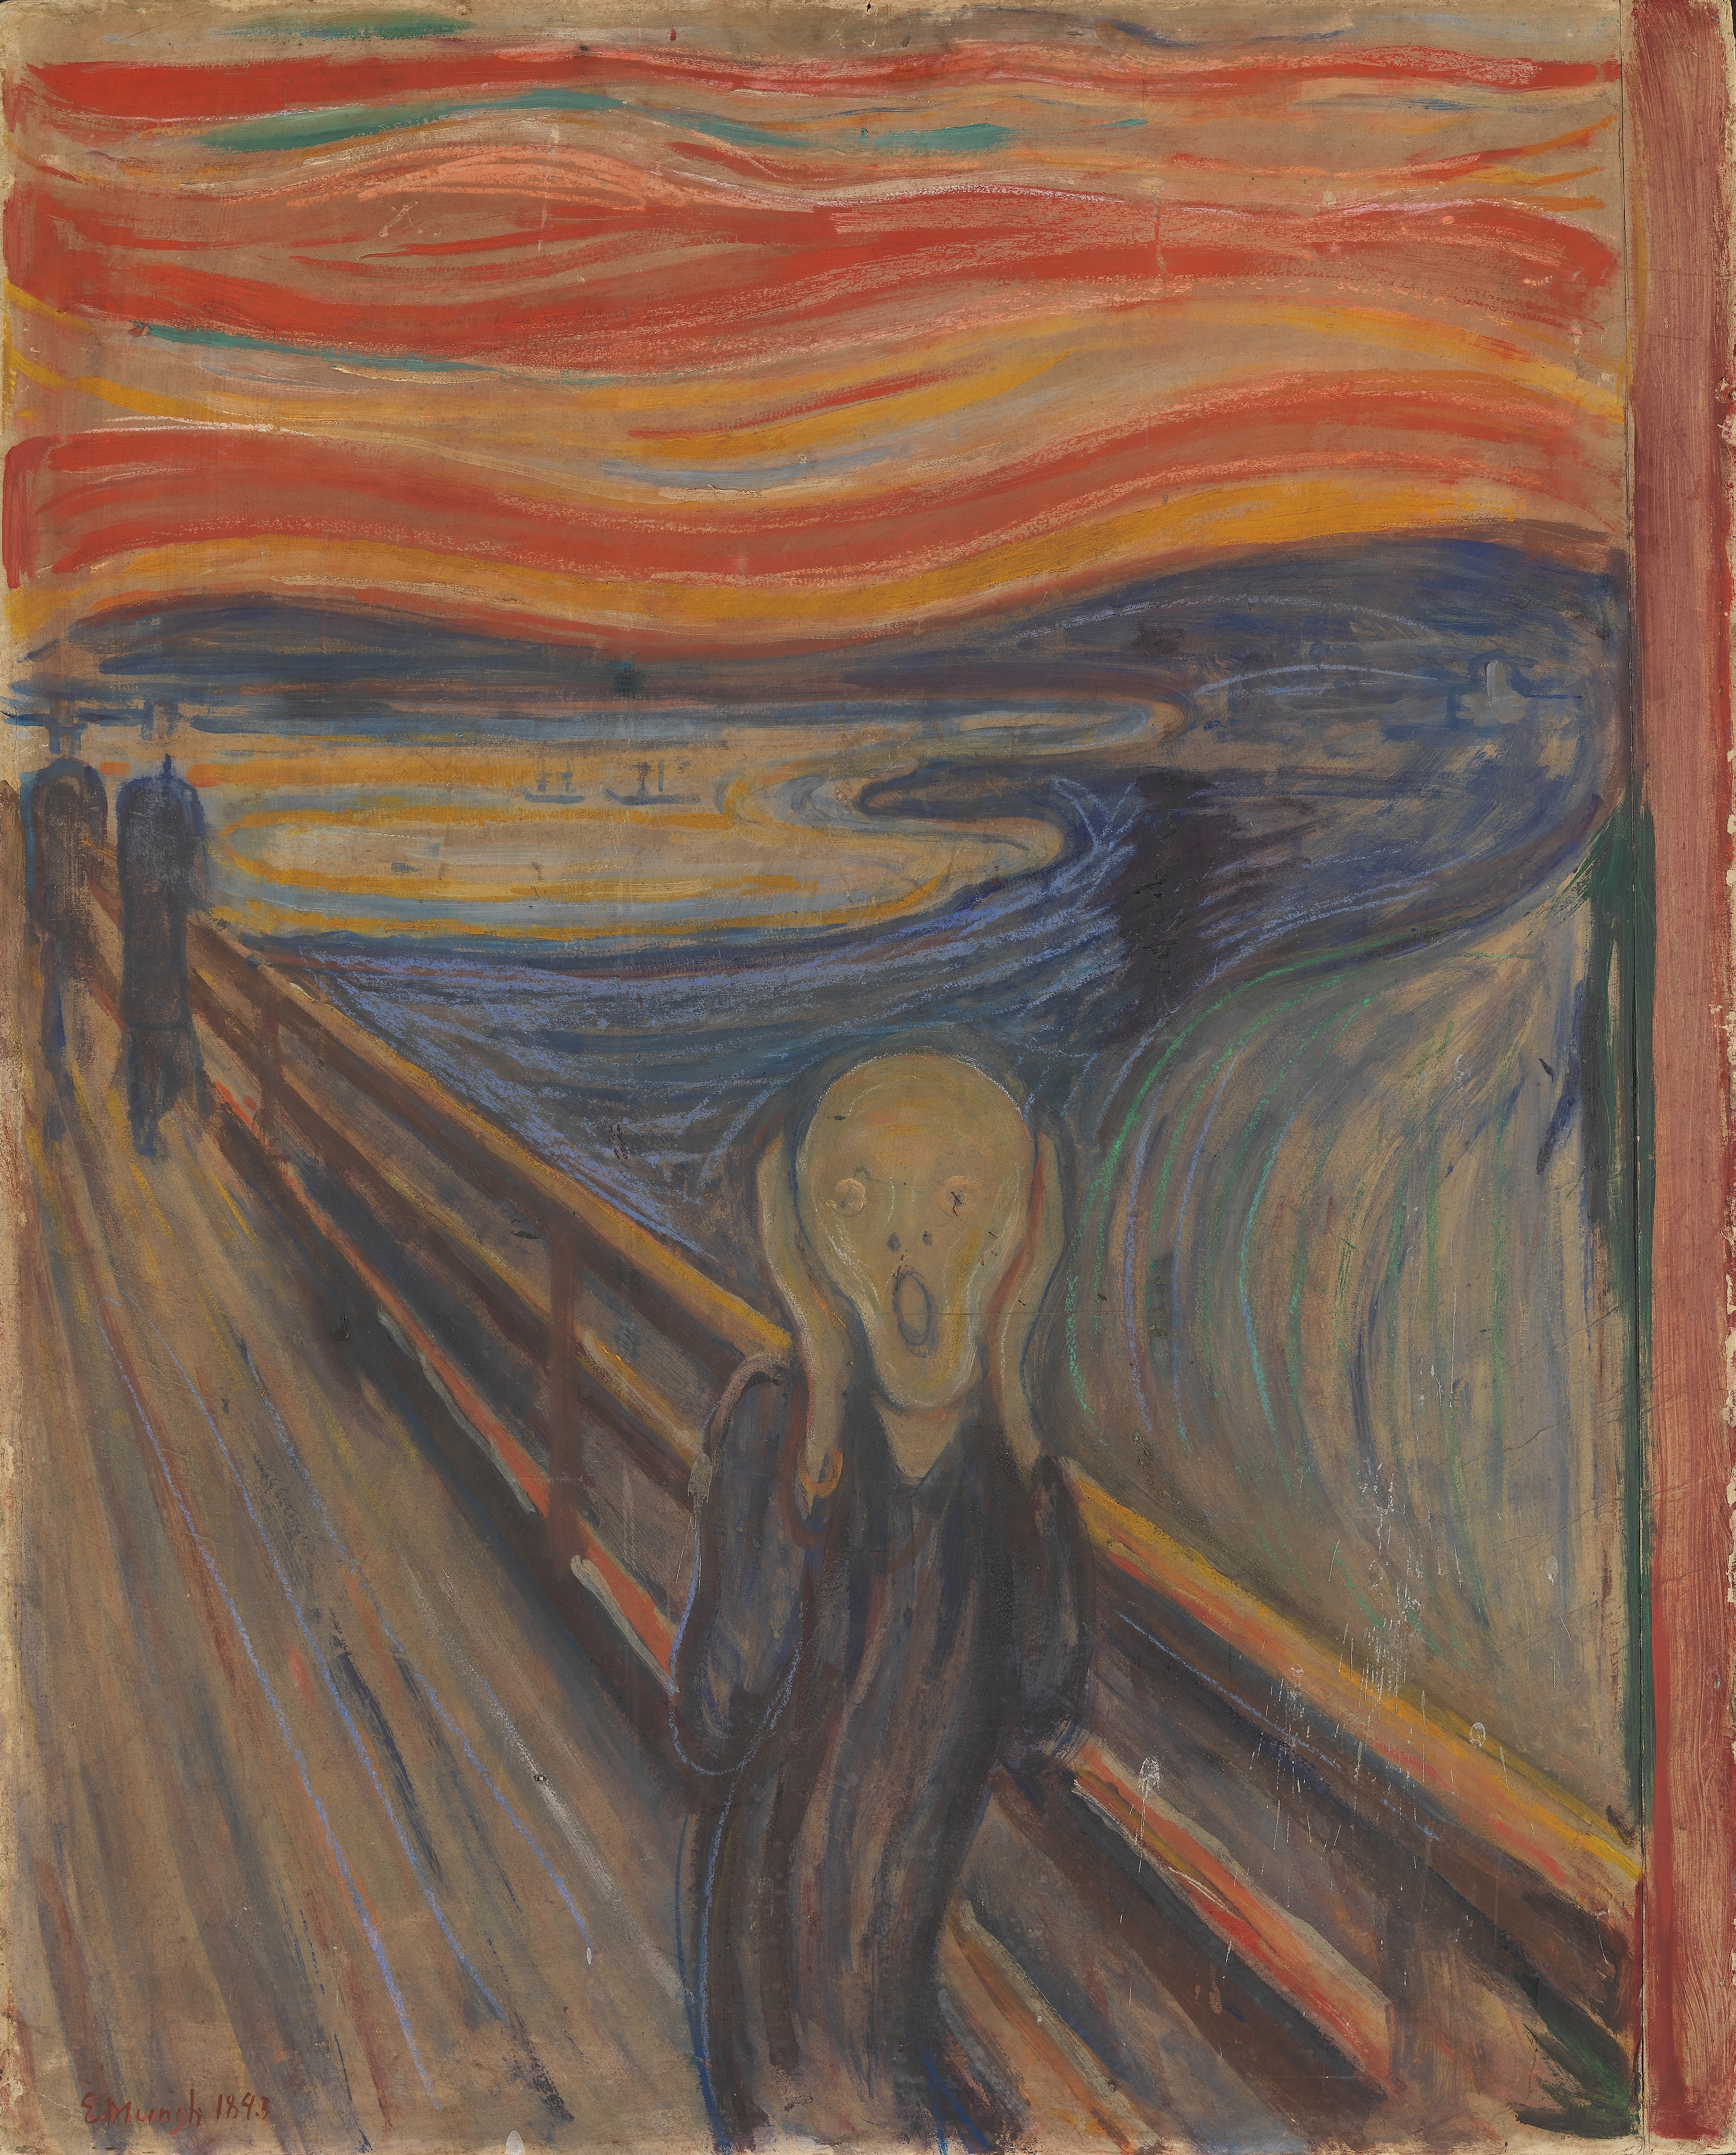
\includegraphics[width=\textwidth]{resources/content/style/the_scream.jpg}
        \end{subfigure}
        \caption{HTW kombiniert mit \textit{The Scream} \cite{the_scream_img}}
    \end{figure}
\end{frame}

\begin{frame}
    \frametitle{Stärkere Gewichtung des $ L_{style} $}

    \begin{figure}[H]
        \centering
        \begin{subfigure}[h]{0.49\textwidth}
            \centering
            \includegraphics[width=\textwidth]{resources/content/experiments/a__the_scream__768x768__style-weight_1e+06__tv-weight_0e+00.jpg}
        \end{subfigure}
        \begin{subfigure}[h]{0.49\textwidth}
            \centering
            \includegraphics[width=\textwidth]{resources/content/experiments/a__the_scream__768x768__style-weight_1e+09__tv-weight_0e+00.jpg}
        \end{subfigure}
        \caption{\textit{The Scream} mit $ \alpha = 1 $, $ \beta = 10^{6} $ und $ \beta = 10^{9} $, $ \gamma = 0 $}
    \end{figure}
\end{frame}

\begin{frame}
    \frametitle{Netzwerke}

    \begin{itemize}
        \item Training 16 verschiedener Netzwerke \pause
        \item $ m = {4, 8, 16, 32} $
        \item $ s = {2, 3, 4, 5} $
    \end{itemize}
\end{frame}

\begin{frame}
    \frametitle{Loss: The Scream}

    \begin{figure}[H]
        \centering
        \includegraphics[width=1.00\textwidth]{resources/content/experiments/fast_loss_plot_experiment2.jpg}
        \caption{Loss: The Scream}
        \label{img:results_the_scream}
    \end{figure}    
\end{frame}

\begin{frame}
    \frametitle{Geräte}
    
    \begin{itemize}
        \item Dell XPS 15 9550
        \item Jetson TX2 \pause
        \item Alle Netzwerke außer $ m = 32 $ können mit Full HD auf Jetson TX2 ausgeführt werden
    \end{itemize}
\end{frame}